%%%%%%%%%%%%%%%%%%%%%%%%%%%%%%%%%%%%%%%%%%%%%%%%%%%%%%%%%%%%%%%%%%%%%%%%
\chapter{Tools and libraries}
\label{ch:tools-and-libraries}
%%%%%%%%%%%%%%%%%%%%%%%%%%%%%%%%%%%%%%%%%%%%%%%%%%%%%%%%%%%%%%%%%%%%%%%%

In this chapter we describe the tools and libraries that we used to
implement the set of experiments described in Chapter
\ref{ch:robust-networks}. This chapter is organized as follows: Section
\ref{sec:tensorflow} is dedicated to
TensorFlow\footnote{https://www.tensorflow.org/} and its computational
graph; Section \ref{sec:keras} is for Keras, a high-level API for
TensorFlow; Section \ref{sec:cleverhans} describes CleverHans, a
library to generate adversarial examples; Section \ref{sec:sklearn}
talks about Scikit-learn, a library for building and training Machine
Learning models, while Section \ref{sec:google-cloud-platform} briefly
mentions Google Cloud Platform, a service by Google that allows you to
buy computational power to run your own code.

\section{TensorFlow}
\label{sec:tensorflow}

\begin{figure}
  \begin{minted}{python}
    >>> import tensorflow as tf
    >>> symbol = tf.constant(42)
    >>> symbol
    <tf.Tensor 'Const:0' shape=() dtype=int32>
  \end{minted}
  \caption{Building a \emph{constant} tensor}
  \label{fig:fortytwo}
\end{figure}

TensorFlow is a C++ framework for Machine Learning released by Google.
It uses a peculiar programming model called Data Flow that allows
parallel and distributed computations, although it can be quite
daunting to use when tinkering. In fact, operations to perform on data
are first described and executed only at a later time. We believe this
can be counter-intuitive for most people. For example, during the
execution of the code shown in Figure \ref{fig:fortytwo}, the variable
\texttt{symbol} doesn't contain a reference to the integer 42 --- as
opposed to what would have been if \texttt{symbol} was an \texttt{int}
variable. Instead, it contains a reference to a node of a
\emph{computational graph} (a description of the computation to perform
on data in terms of nodes and edges) which will always output 42. In
TensorFlow, computation is done by connecting one or more of these nodes
to other nodes, letting \emph{tensors} (the object that you manipulate
in TensorFlow) \emph{flow} around this
graph (in case of Figure \ref{fig:fortytwo}, the tensor is the output
of the only one node in the graph: the tensor is 42). Problem is that,
in general, it's hard to
determine beforehand what is going to be the value of a tensor, that is the
\emph{output} of the computational graph. This is slowing down
exploratory analysis.

\begin{figure}
  \centering
  \begin{tikzpicture}[>=latex,line join=bevel,]
  \node (a) at (27.0bp,72.0bp) [draw,ellipse] {a}; \node
  (add) at (117.95bp,45.0bp) [draw,ellipse] {add}; \node (b)
  at (27.0bp,18.0bp) [draw,ellipse] {b}; \draw [->] (b)
  ..controls (61.417bp,28.218bp) and (72.527bp,31.516bp) ..
  (add); \draw [->] (a) ..controls (61.417bp,61.782bp) and
  (72.527bp,58.484bp) .. (add);
  \end{tikzpicture}
  \caption[]{One of the simplest computational graph possible.}
  \label{fig:easy-graph}
\end{figure}

By the way, TensorFlow's computational graphs are a fundamental part of
the framework. A computational graph is a directed graph representing a
computation involving tensors. A tensor in TensorFlow is a generalized
multi-dimensional array: it can be a scalar, a matrix, a batch of RGB
images (which is a 4D vector\footnote{If you always thought humans
  can't visualize four dimensions all at once, think of this
  example.}), etc. Each node represents an operation on tensors, while
edges represent tensors.

For example, Figure \ref{fig:easy-graph} shows a very simple
computational graph. It's the one associated to an addition of two
\emph{numerical} tensors (two tensors made of numbers: two
\texttt{tf.float32}, two \texttt{tf.int64}, etc.): the first two nodes
\texttt{a} and \texttt{b} output one tensor each; those are used to
feed the \texttt{add} node that will output the tensor resulting from
the sum of \texttt{a} and \texttt{b}.

\begin{figure}
  \centering
  \begin{tikzpicture}[>=latex,line join=bevel,]
    \node (s3) at (27.0bp,90.0bp) [draw,ellipse] {};
    \node (s2) at (243.0bp,90.0bp) [draw,ellipse] {};
    \node (s1) at (171.0bp,90.0bp) [draw,ellipse] {};
    \node (s4) at (99.0bp,90.0bp) [draw,ellipse] {};
    \node (d4) at (99.0bp,18.0bp) [draw,ellipse] {};
    \node (d2) at (243.0bp,18.0bp) [draw,ellipse] {};
    \node (d3) at (27.0bp,18.0bp) [draw,ellipse] {};
    \node (d1) at (171.0bp,18.0bp) [draw,ellipse] {};
    \draw [->] (s1) ..controls (171.0bp,64.131bp) and (171.0bp,54.974bp)  .. (d1);
    \draw [->] (s2) ..controls (196.78bp,66.889bp) and (157.24bp,47.119bp)  .. (d4);
    \draw [->] (s3) ..controls (89.947bp,69.018bp) and (165.24bp,43.919bp)  .. (d2);
    \draw [->] (s1) ..controls (145.8bp,64.803bp) and (132.68bp,51.685bp)  .. (d4);
    \draw [->] (s4) ..controls (124.2bp,64.803bp) and (137.32bp,51.685bp)  .. (d1);
    \draw [->] (s2) ..controls (243.0bp,64.131bp) and (243.0bp,54.974bp)  .. (d2);
    \draw [->] (s3) ..controls (52.197bp,64.803bp) and (65.315bp,51.685bp)  .. (d4);
    \draw [->] (s4) ..controls (145.22bp,66.889bp) and (184.76bp,47.119bp)  .. (d2);
    \draw [->] (s2) ..controls (180.05bp,69.018bp) and (104.76bp,43.919bp)  .. (d3);
    \draw [->] (s4) ..controls (73.803bp,64.803bp) and (60.685bp,51.685bp)  .. (d3);
    \draw [->] (s3) ..controls (27.0bp,64.131bp) and (27.0bp,54.974bp)  .. (d3);
    \draw [->] (s3) ..controls (73.222bp,66.889bp) and (112.76bp,47.119bp)  .. (d1);
    \draw [->] (s2) ..controls (217.8bp,64.803bp) and (204.68bp,51.685bp)  .. (d1);
    \draw [->] (s1) ..controls (124.78bp,66.889bp) and (85.238bp,47.119bp)  .. (d3);
    \draw [->] (s1) ..controls (196.2bp,64.803bp) and (209.32bp,51.685bp)  .. (d2);
    \draw [->] (s4) ..controls (99.0bp,64.131bp) and (99.0bp,54.974bp)  .. (d4);
  \end{tikzpicture}
  \caption[neural-network]{Feedforward neural network with only input
    and output layer}
  \label{fig:neural-network}
\end{figure}

The most commonly used way to program the computational graph is by
using an API for the Python language. A perhaps interesting example of
the kind of computation one can express in TensorFlow using Python
would the implementation of a neural network. Figure
\ref{fig:neural-network} graphically represents the network
we're going to implement: a simple feedforward network of four input
neurons and four output neurons. As explained in Chapter
\ref{ch:background}, each layer in a feedforward neural network performs
a linear operation on its input and apply an activation function on
that result. That is, it computes

\[ \text{activation}(X * W + b) \]

given its weight matrix and its bias vector, \( W \in \mathbb{R}^{4
  \times 4} \) and \( b \in \mathbb{R}^{4}\) respectively, while
\( \text{activation} \) is a \emph{non}-linear function such as
the rectifier or the softmax function.

\begin{figure}
  \begin{minted}{python}
    >>> import tensorflow as tf
    >>> W = tf.random_normal(shape=(4, 4))
    >>> b = tf.random_normal(shape=(4,))
    >>> X = tf.placeholder(shape=(None, 4), dtype=tf.float32)
    >>> logits = tf.matmul(X, W) + b
    >>> probabilities = tf.nn.softmax(logits)
    >>> probabilities
    <tf.Tensor 'Softmax:0' shape=(?, 4) dtype=float32>
  \end{minted}
  \caption{TensorFlow commands to generate a feedforward network}
  \label{fig:tensorflow-feedforward}
\end{figure}

To get an idea of how to do that in TensorFlow see Figure
\ref{fig:tensorflow-feedforward}, where $W$ and $b$ are initialized
drawing values from a standard normal distribution. Note that
\texttt{X} is a \emph{placeholder}: it is a TensorFlow way to make room
in the graph for something whose value will be provided later. In
Figure \ref{fig:tensorflow-feedforward} that function is applied to the
\emph{logit}\footnote{https://datascience.stackexchange.com/a/31045/50780},
i.e. the output of the matrix multiplication. As explained in Chapter
\ref{ch:background} this is done for various reasons but one of the
simplest ones is that it squashes the output of the network in $[0,1]$
allowing to interpret it in terms of confidence levels --- see Chapter
\ref{ch:background}.

\begin{figure}
  \begin{minted}{python}
    >>> import numpy as np
    >>> batch = np.random.rand(10, 4)
    >>> batch
    >>> array([[0.54485176, 0.33854871, 0.45185129, 0.79884188],
      [0.41204776, 0.23552753, 0.04101023, 0.47883844],
      [0.25544491, 0.7610509 , 0.49307137, 0.6098213 ],
      [0.02545156, 0.70459456, 0.22067103, 0.64743811],
      [0.92359354, 0.96497353, 0.45790538, 0.49380769],
      [0.13330072, 0.22947966, 0.02996348, 0.69954114],
      [0.38397249, 0.30473362, 0.87023559, 0.90153084],
      [0.77056319, 0.94843128, 0.39095345, 0.50572861],
      [0.90112077, 0.19240995, 0.48437166, 0.46200152],
      [0.98589042, 0.2013479 , 0.86091217, 0.55886214]])
    >>> with tf.Session() as session:
    ...     session.run(probabilities, feed_dict={X: batch})
    ...
    >>> array([[0.03751625, 0.8651346 , 0.05245555, 0.04489357],
      [0.11873736, 0.6301607 , 0.17646323, 0.07463871],
      [0.06252376, 0.82338244, 0.07284217, 0.04125158],
      [0.12086256, 0.6911012 , 0.14362463, 0.04441159],
      [0.03662292, 0.8575108 , 0.04834893, 0.05751737],
      [0.12984137, 0.63064647, 0.1834405 , 0.05607158],
      [0.01711418, 0.93650085, 0.02116078, 0.02522417],
      [0.04886489, 0.83023334, 0.06332602, 0.05757581],
      [0.033136 , 0.84808177, 0.05061754, 0.06816475],
      [0.01250888, 0.9262628 , 0.01797607, 0.0432523 ]], dtype=float32)
  \end{minted}
  \caption{Running a computational graph within a session}
  \label{fig:use-session}
\end{figure}

\begin{figure}
  \begin{minted}{python}
    >>> W = tf.Variable(W)
    >>> b = tf.Variable(b)
    >>> logits = tf.matmul(X, W) + b
    >>> # redefine logits using variables 
    >>> probabilities = tf.nn.softmax(logits)
  \end{minted}
  \caption{Making variables out of \texttt{W} and \texttt{b}}
  \label{fig:making-variables}
\end{figure}

Now, to get results out of the graph you need what's called a
\emph{session} in TensorFlow. Basically, a session \emph{powers on} the
graph, allowing you to run the computational graph with your own data
and get actual tensors of actual numbers out of it. Of course building
neural networks is pretty useless if you can't train them: at first the
whole output is only based on the random weights and biases randomly
extracted from a normal distribution --- for example, probabilities in
Figure \ref{fig:use-session} are totally non-sense: there's no training
set and no training phase yet.

To train a network in TensorFlow we need a \texttt{tf.Variable}. A
variable in TensorFlow is a tensor which can be modified by sessions,
whose value persists across them. This allows you to basically add
parameters to your computational graphs, allowing to iteratively
\emph{change} them. Using a learning procedure that modifies the
\texttt{tf.Variable}s to reduce the distance from the target function
to the actual function computed by the network, makes the model
\emph{learning}. In the current example, the part of the graph that you
want the learning procedure to modify are the tensors $W$ and $b$. As
in Figure \ref{fig:making-variables} to build a \texttt{tf.Variable} in
TensorFlow you can just wrap those tensors.

\begin{figure}
  \begin{minted}{python}
    >>> from tf.nn import tf_cross_entropy
    >>> y_true = tf.placeholder(shape=(None,), dtype=tf.float32)
    >>> cross_entropy = tf_cross_entropy(logits=logits, labels=y_true)
  \end{minted}
  \caption{Creating the cross-entropy operation}
  \label{fig:cross-entropy}
\end{figure}

\begin{figure}
  \begin{minted}[linenos]{python}
    from tf.train import GradientDescentOptimizer as SGD
    optimizer = SGD(learning_rate=0.5).minimize(cross_entropy)

    with tf.Session() as session:
        session.run(tf.global_variables_initializer())

    n_training_steps = 10
    for i in range(n_training_steps):
        images, classes = next_batch()

        with tf.Session() as session:
            session.run(optimizer, feed_dict={X: images,
                                              y_true: classes})
  \end{minted}
  \caption{Training a feedforward neural network built with TensorFlow}
  \label{fig:training-network}
\end{figure}

The last thing we want to do before abandoning this example is the
actual training. To perform training we need a training set. As
explained in Chapter \ref{ch:background}, a training set consists of a
bunch of data and a label associated to each input, representing the
class of that data. As \emph{training} basically means minimizing a
loss function, we need that function: as in Figure
\ref{fig:cross-entropy}, we're using the cross-entropy function.
Cross-entropy is defined as

\[ H(p, q) = - \sum_i {p_i \, \log{q_i}} \]

where $p$ and $q$ are two probability distributions. In our case, $p$
is the \emph{probability} distribution for an input (the classifier's
confidence levels, the output of a neural network if the model is a
neural network), and $q$ is the one-hot encoding of the actual class of
the input (which looks and it's in fact used here as a probability
distribution).

\begin{figure}
  \centering
  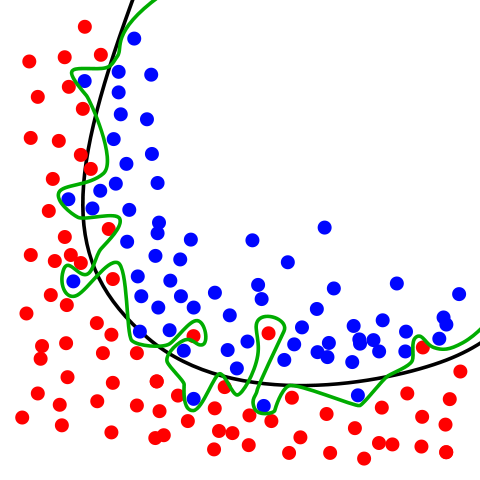
\includegraphics[width=0.5\linewidth]{wikipedia-overfitting.png}
  \caption{Green curve represents an overfitting classifier. By
    Chabacano [CC BY-SA 4.0
      (https://creativecommons.org/licenses/by-sa/4.0)], from Wikimedia
    Commons}
  \label{fig:wikipedia-overfitting}
\end{figure}

The gradient descent algorithm is then used to iteratively do the job.
TensorFlow implements the procedure via
\texttt{GradientDescentOptimizer.minimize(loss)} that returns an
operation that each time you run in a session will modify the graph's
\texttt{tf.Variable}s, aiming to lower the value of the cross-entropy
\emph{loss} function. We can build a loop to train the network over and
over again, as in Figure \ref{fig:training-network}. This will push the
loss function toward a local minimum; hopefully a useful one, i.e. a
minimum that corresponds to good results even on data outside the
training set. Otherwise the model is said to \emph{overfit}. That is,
the model \emph{fit} so well over the training set that fail generalize
to the whole input space. For example, in Figure
\ref{fig:wikipedia-overfitting} we have plotted two classifiers: one
drawn as a green curve, the other as a black curve. The \emph{green}
model has a better accuracy (that is, it has a high rate of correct
classifications) on the training set, but its characteristics are
clearly so much dependent on the set the models has been trained that
it will almost surely fail to keep that high accuracy on data outside
the training set --- while the \emph{black} model has a higher
probability to be a good model.

\section{Keras}
\label{sec:keras}

\begin{figure}
  \begin{minted}[linenos]{python}
    from keras.engine.base_layer import Layer
    import tensorflow as tf

    class Add42(Layer):
        def __init__(self):
            self.fortytwo = tf.constant(42)

        def __call__(self, X):
            return tf.add(X, self.fortytwo)

    model = Sequential([Dense(...), Add42(), ...])
  \end{minted}
  \caption{A toy-example for a Keras layer}
  \label{fig:toy-layer}
\end{figure}

Keras\footnote{https://keras.io/} is a library for building Machine
Learning models using a simple API that abstracts away the interface of
a backend of choice, e.g. TensorFlow. When you use the library, you're
encouraged to manipulate \emph{layers} instead of plain tensors. In
fact the whole concept of \emph{tensors} is hidden away by the library.
To implement your model you're expected to stack layers one on top the
other, expressing a \emph{sequential} manipulation of the
data\footnote{https://keras.io/\#getting-started-30-seconds-to-keras}.
Under the hood, a \texttt{Layer} is simply a callable object whose
\texttt{\_\_call()\_\_} method takes a TensorFlow tensor \texttt{X} and
manipulates it --- see Figure \ref{fig:toy-layer}.

\begin{figure}
  \begin{minted}{python}
    >>> from keras.models import Sequential
    >>> model = Sequential([
    ... Dense(batch_input_shape=(None, 4), units=4),
    ... Activation('softmax')])
  \end{minted}
  \caption{Feedforward network using Keras layers}
  \label{fig:feedforward-with-layers}
\end{figure}

As shown in Figure \ref{fig:feedforward-with-layers}, to implement the
simple feedforward neural network of Figure
\ref{fig:wikipedia-neural-network} one would stack a \texttt{Dense}
layer of 4 hidden neurons and an \texttt{Activation} layer implementing
the softmax function. Compare that to the TensorFlow implementation we
did in Section \ref{sec:tensorflow} and you'll realize how much easier
is to read it and to think about it.

This nicer API that allows to immediately think about model's
architecture has the cost of an abstraction level that at the time of
this writing in our opinion is not enough stable to allow programmers
to be completely oblivious of the original backend --- in my case
TensorFlow.

\section{CleverHans}
\label{sec:cleverhans}

CleverHans\footnote{https://www.cleverhans.io/} is a library for
building adversarial examples written by Google, OpenAI and
Pennsylvania State University. It implements a variety of
attacks\footnote{https://cleverhans.readthedocs.io/en/latest/source/attacks.html}
including fast gradient sign (see Chapter \ref{ch:background})
against neural networks and it's compatible with models built with
Keras or just plain TensorFlow. It leverages the computational graphs
of TensorFlow to generate adversarial examples, so using the
library without knowing TensorFlow is not easy.

\begin{figure}
  \begin{minted}[linenos]{python}
  from cleverhans.attacks import FastGradientMethod
  from cleverhans.utils_keras import KerasModelWrapper

  # `model` is a Keras model
  cleverhans_model = KerasModelWrapper(model)
  attack = FastGradientMethod(cleverhans_model)

  example_sym = attack.generate(model.input, **kwargs)
  # example_sym will give the adversarial examples
  # when run in a session.
  \end{minted}
  \caption{Generating adversarial examples using CleverHans}
  \label{fig:cleverhans-attack-dot-generate}
\end{figure}

To generate adversarial examples for a given model CleverHans needs to
be able to read some internals of the model --- inputs are generated in
a white-box approach. CleverHans already provides a couple of utilities
to do that \emph{model inspection} --- e.g. for Keras there's a
\texttt{KerasModelWrapper}\footnote{https://github.com/tensorflow/cleverhans/blob/66125be/cleverhans/utils\_keras.py\#L101}
--- transforming the model into an object that CleverHans is able to
handle. Once a model has the interface CleverHans expects, it's
possible to choose the attack technique via classes inhereting from the
same \texttt{Attack} class. They are all exposing a \texttt{generate}
method that will return a node of the corresponding computational
graph; when you run it in a session it will return the related
adversarial examples. See Figure
\ref{fig:cleverhans-attack-dot-generate} for a short example.

\section{Scikit-learn}
\label{sec:sklearn}

scikit-learn is a Python library written by David Cournapeau providing
a number of models, learning algorithms and data manipulation utilities
for Machine Learning. It's pretty popular for fast prototyping as it
uses a simple and consistent API, with the ability to handle numpy
arrays or even Python lists --- instead of having to learn about the
computational graph.

We've used scikit-learn to reuse a couple of decomposition
algorithms\footnote{http://scikit-learn.org/0.20/modules/classes.html\#module-sklearn.decomposition}
without having to implement them. This required a bit of thinking as
while Keras and TensorFlow use a lot the computational graph,
scikit-learn is completely oblivious of that structure.

\begin{figure}
  \begin{minted}[linenos]{python}
  import sklearn.decomposition
  pca = sklearn.decomposition.PCA(n_components=100)
  pca.fit(training_set)

  batch = next_batch()
  filtered_batch = pca.inverse_transform(pca.transform(batch))
  \end{minted}
  \caption{Using \texttt{sklearn.decomposition.PCA} to get a
    \emph{filtered} image}
  \label{fig:transform-inverse_transform}
\end{figure}

The way I've used scikit-learn decomposition algorithm has been by
leveraging classes exposing both a \texttt{transform(X)} and a
\texttt{inverse\_trasform(X)}. This way I built \emph{filters} that
\emph{reduced} the amount of information in the original data. See
Figure \ref{fig:transform-inverse_transform}.

\section{Google Cloud Platform}
\label{sec:google-cloud-platform}

\begin{figure}
  \centering
  \begin{tabular}{|c|c|}
    \hline
    CPU platform & Intel Haswell \\
    \hline
    memory & 60 GB \\
    \hline
    vCPUs & 16 \\
    \hline
    GPU & 1 x NVIDIA Tesla P100 \\
    \hline
  \end{tabular}
  \caption{Information of the machine used via GCP.}
  \label{fig:expensive-machine}
\end{figure}

Google Cloud Platform is a set of services that allows people to buy
computational power from Google. In our case, we used GCP to get access
to a GPU for few dollars a
month\footnote{https://cloud.google.com/blog/products/gcp/introducing-improved-pricing-for-preemptible-gpus}.
Since we had \$300 of free credit we chose an expensive machine type as
described in Figure \ref{fig:expensive-machine}. That made running
experiments a lot faster in many cases.

\begin{figure}
  \begin{minted}{text}
  [g@x220 ~]$ gcloud compute ssh root@bowser -- -X
  No zone specified. Using zone [us-east1-b] for instance: [bowser].
  Welcome to Ubuntu 16.04.5 LTS (GNU/Linux 4.15.0-1014-gcp x86_64)

  * Documentation:  https://help.ubuntu.com
  * Management:     https://landscape.canonical.com
  * Support:        https://ubuntu.com/advantage

    Get cloud support with Ubuntu Advantage Cloud Guest:
      http://www.ubuntu.com/business/services/cloud

  0 packages can be updated.
  0 updates are security updates.


  Last login: Thu Sep 27 15:35:52 2018 from 79.24.139.192
  root@bowser:~# 
  \end{minted}
  \caption{Using \texttt{gcloud} to connect via ssh to Google remote \emph{machine}}
\end{figure}
